
\documentclass{article}
\usepackage[margin=1in,footskip=0.25in]{geometry}
\usepackage{fancyhdr}
\usepackage{graphicx}
\usepackage{multirow}
\usepackage{adjustbox}
\usepackage{graphicx}
\usepackage{hyperref}
\usepackage{longtable}
\usepackage{booktabs}
\usepackage{array}
\usepackage[table]{xcolor}
\usepackage[ backend=biber, style=authoryear ]{biblatex} \addbibresource{references.bib}
\usepackage{tabularx}
\usepackage{url}

\setlength{\bibitemsep}{0.5\baselineskip}
\linespread{1.2}

\begin{document}

\begin{titlepage}
    \begin{center}
        \vspace*{1cm}

        {\Huge\bfseries TSML Proposal \par}
        \vspace{0.5cm}
        {\Large COMP60055\par}

        \vspace{1.5cm}
        {\large\bfseries Michal Litwin \par}
        \large
        RICOH UK Products Ltd\\
        Staffordshire University

        \vfill

        {\large \textbf{Workplace Supervisor:} Claire Shepherd \par}
        \vspace{0.8cm}

        \large Software Engineering Route\\

    \end{center}
\end{titlepage}

\tableofcontents
\pagebreak
\listoftables
\pagebreak
\listoffigures
\pagebreak

\section{Introduction}
Ricoh UK Products Ltd is a leading provider of products and goods, focusing on toner printing and recycling.
IoT Digital Operations department deploys software solutions to meet company improvements and objectives.
Server side web applications are Currently hosted on on-premis IIS (Internet Inforamtion Services) servers.
However, the organisation requests a migratation to imrpove response rate for stakeholders, use more compatible software, incorporate automation, improve performance and more.
\\

\subsection{Organisation Background}
RPL (Ricoh Products Ltd), established in 1983, is a United Kingdom arm of the larger Japanese Ricoh group.
RPL provide print solutions, ink supplies and technical services. 

\subsubsection{Business Vision, Mission \& Value}



\subsubsection{Business Aims and Objectives}


\pagebreak{}
\section{Transformation Necessity}
\subsection{Problem}
mention the top 5 issues, rank them. 

\subsubsection{Situation}

\subsection{Requirements}
bla bla bla

research, hosting provider. 
week 1 - business values, strategy. look at org, values, missions, aim, objectives. put in appendix, and summarise in intro section

identify the core objectives/mission company has stated, which represent what im doing. alligning with company.

in the beginning, three business theories, classical org, system theory, and choose another theory.

things you would if thorry used, classical theory - lots of management, pyramid. last column, launch week

definition, indicator, is visible in company

bussiness impact in problem section. 

just use swot. summarise petsle in take home message. only if needed. integrate law or policy.

issues are explained in business impact table. 


\pagebreak{}
\section{Proposed Solution}
\subsection{Options Considered}
\subsection{Recommendations}
\subsubsection{Link to Business and Digital Strategy}
\subsubsection{Expected Position}

\pagebreak{}
\section{Project Management}
decision matrix in here?
\subsection{Scope and Objectives}
\subsection{Costing}
\subsection{Project Approach}
\subsection{Risk Management}
\subsection{Work Breakdown Structure}
\subsection{Road Map}

\section{Business Case}
\subsection{Improvement to competitive advantage}
\subsection{Legal, Ethical, Social and Professional Standards}
\subsection{Sustainability}

\pagebreak
\section{Appendices}

\subsection{Classical Organisation Theory}
Classical Organisation Theory analysis an organisaton's structure and management to coordinate focus and improve efficiency. 
Ricoh UK Products Ltd contains a clear hierarchical structure through designated job roles and departments that focus on related core processes.
Each department is responsible for its assigned tasks, contributing to overall business growth and direction. 
\\

Figure \ref{fig:OrgStructure}  displays the core Ricoh Products Ltd organisational structure and hierarchy, contributing to overall production efficiency.

\vspace{0.5cm}
\begin{figure}[h]
    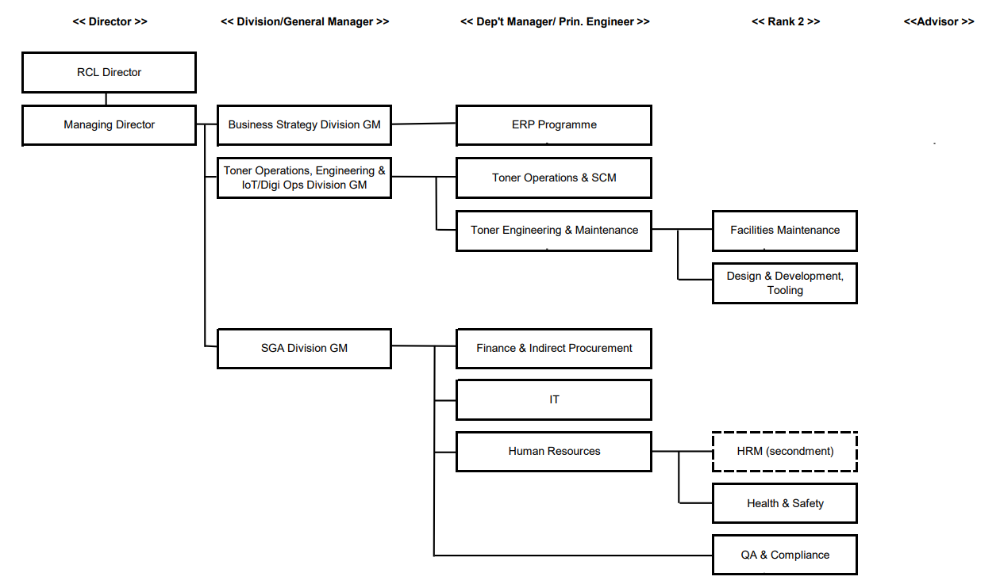
\includegraphics[width=\textwidth]{media/Classical Organisation Structure.png}
    \centering
    \caption{Organisational Structure}
    \label{fig:OrgStructure}
\end{figure}
\vspace{0.5cm}

As illustrated in the above figure, Ricoh Products Ltd, assigns and groups departments under direct supervision ensuring targets and goals are met.
Roles are split into ranks and titles, including Directors, General Managers and Department Managers, each with its associated rank level.

\pagebreak{}
\subsection{Organisation System Theory}

Organisation System Thoery views a corporation as an embedded system with interrelated groups working together towards a common goal.
This theory incorporates departments, people, technology as well as exterior factors.
One change in a given area affects other areas working closely with the origin.
\\

Figure \ref{fig:SystemTheory} below displays Ricoh UK Product's Ltd organisational system and cycle, influenced by inputs and feedback from its outputs.

\vspace{0.5cm}
\begin{figure}[h]
    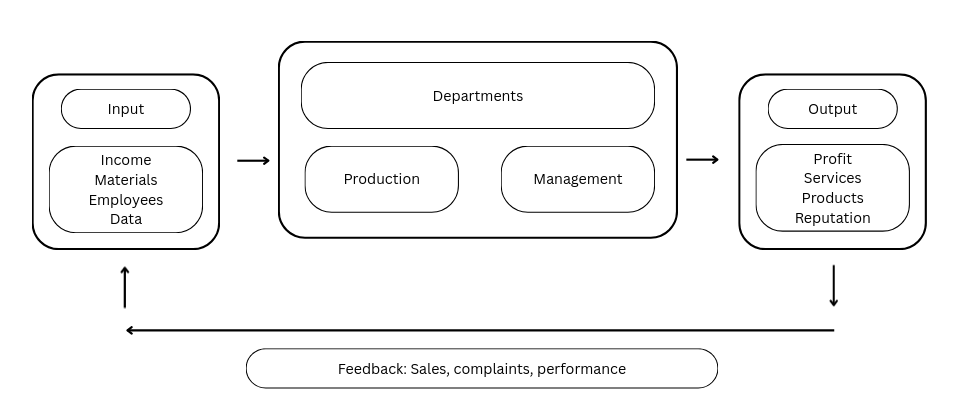
\includegraphics[width=\textwidth]{media/System Theory.png}
    \centering
    \caption{Organisational Structure}
    \label{fig:SystemTheory}
\end{figure}
\vspace{0.5cm}

Evidenced aboce in Figure \ref{fig:SystemTheory}, Ricoh UK Products Ltd incroporates feedback from sales and performance metrics, to adjust inputs, goals and objectives assigned to departments and production.
As a result, Ricoh systematically adapts to change as a living organism, to improve outputs for increased profit, services and its reputation.
``

\pagebreak{}
\subsection{Action Centred Leadership Theory}
(ACL) Action Centred Leadership explains effective leadership manages areas of need, including Task, Team and Individual.
This method is a functional approach to leadership, attending to organisational tasks, efficiency as well as human relations with employees.
\\

Figure \ref{fig:ActionCentredLeadership} below, pictures the three main categories within Action Centred Leadership.

\vspace{0.5cm}
\begin{figure}[h]
    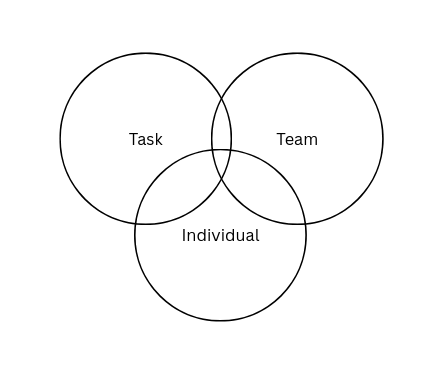
\includegraphics[width=12cm]{media/Action Centred Leadership.png}
    \centering
    \caption{Action Centred Leadership}
    \label{fig:ActionCentredLeadership}
\end{figure}
\vspace{0.5cm}

Ricoh Products Ltd incorporates all three categories showcased in Figure \ref{fig:ActionCentredLeadership} , through deep communication, strategy planning and collobaration.
Departments participate in regular meetings, discussing progress and challenges, whilst department managers arrange personal sessions to privately discuss targets and to gather any feedback.
Business goals and department objectives are shared within teams, ensuring each employee is aware and working towards the company vision. 




% references

\end{document}
